\section{Detailed Class Results}
\label{app:class}
\begin{table}[H]\centering
\caption{Per-class test F1 (\%). Each class has 1,000 test images.
Values are rounded to two decimal places.}
\begin{tabular}{lrrrrr}\toprule
Class & Linear & MLP & CNN & LSTM & Transformer\\\midrule
\tabledata{generated/f1_rows.tex}
\bottomrule\end{tabular}
\end{table}

\begin{table}[H]\centering
\caption{CNN class metrics. Precision, recall and F1 are percentages.
Errors count true-class images assigned another label.}
\begin{tabular}{lrrrr}\toprule
Class & Precision & Recall & F1 & Errors\\\midrule
\tabledata{generated/cnn_class_rows.tex}
\bottomrule\end{tabular}
\end{table}

For class $k$, precision is $TP_k/(TP_k+FP_k)$ and recall is
$TP_k/(TP_k+FN_k)$. The CNN's Shirt recall is 71.80\%, meaning it correctly
classifies 718 of the 1,000 Shirt images. Its Shirt precision is 78.90\%,
meaning that some images predicted as Shirt actually belong to another class.

The exact values are recomputed from the saved confusion counts before
rounding. All classes have equal support, so the mean class recall equals
overall accuracy. This equality does not make precision or F1 redundant.

\clearpage
\section{Additional Confusion Matrices}
The matrices below use the same label mapping and color range as the CNN
matrix. Rows are true labels and columns are predictions. Each row sums to
1,000 and each complete matrix contains 10,000 predictions.

\begin{figure}[H]\centering
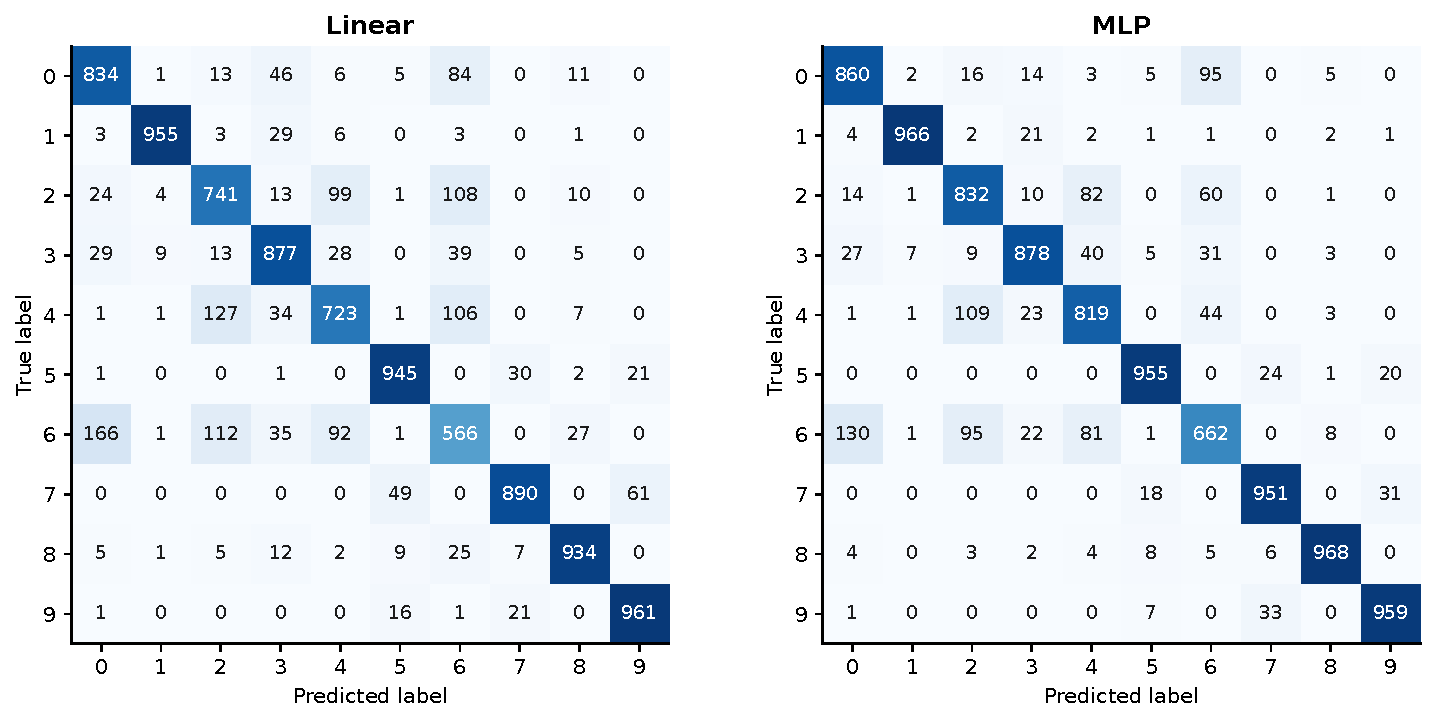
\includegraphics[width=\linewidth]{baseline_confusions.pdf}
\caption{Official-test confusion matrices for the Linear and MLP baselines.}
\end{figure}

\begin{figure}[H]\centering
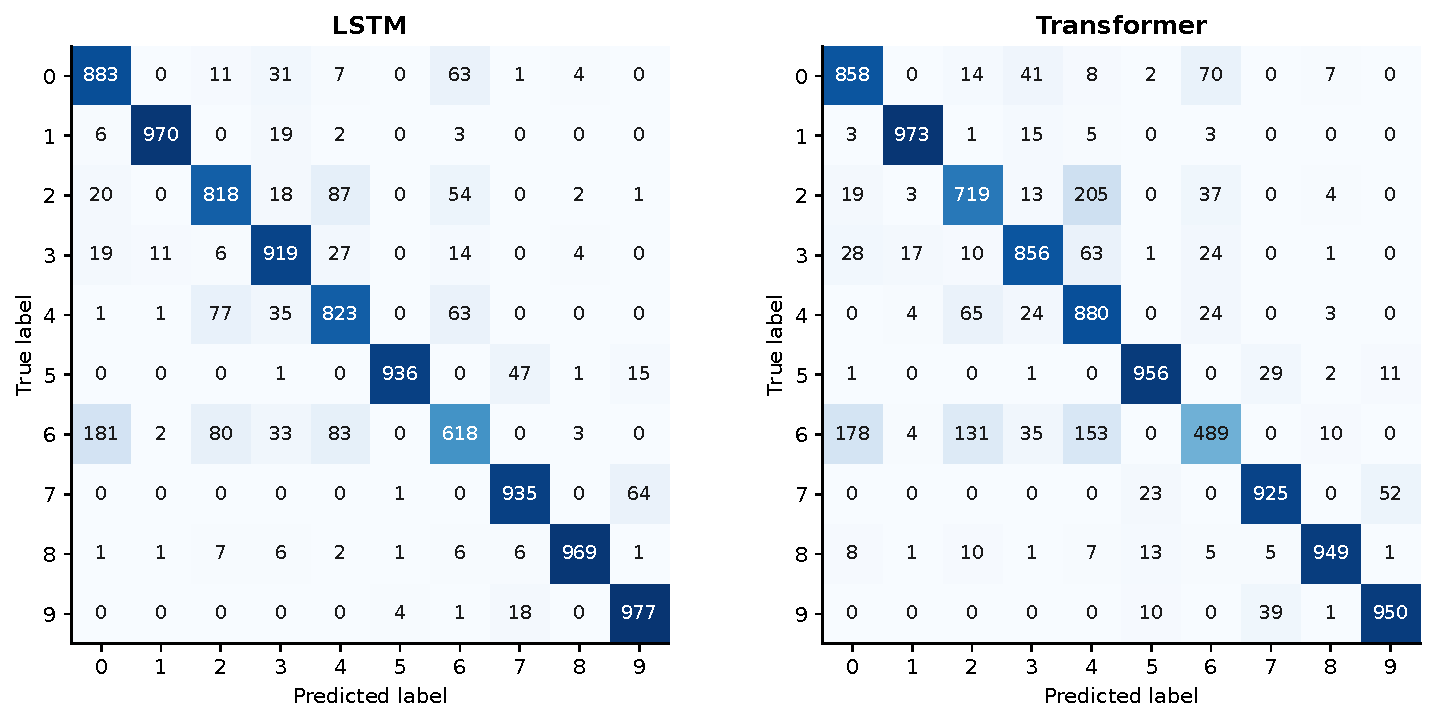
\includegraphics[width=\linewidth]{sequence_confusions.pdf}
\caption{Official-test confusion matrices for the row LSTM and patch Transformer.}
\end{figure}

\small
Labels: 0 T-shirt/top; 1 Trouser; 2 Pullover; 3 Dress; 4 Coat;
5 Sandal; 6 Shirt; 7 Sneaker; 8 Bag; 9 Ankle boot.
\normalsize

\clearpage
\section{Reproducibility and Evidence}
\small
\subsection{Environment and saved files}
The CUDA training and test-evaluation records identify Windows 11,
Python 3.12.10, PyTorch 2.9.1+cu128, torchvision 0.24.1+cu128,
NumPy 2.2.6 and scikit-learn 1.7.2. The GPU is an NVIDIA GeForce
GTX 1660 SUPER with 6 GiB of memory. Linear and MLP computational costs now
come from separate CUDA training and test runs; the original selected
checkpoints remain the source of classification scores and error analysis.

From the repository's \texttt{A1} folder, the principal files are:
\begin{table}[H]\centering\small
\caption{Implementation and experiment evidence.}
\begin{tabularx}{\linewidth}{p{.46\linewidth}X}\toprule
Path & Role\\\midrule
\texttt{a1/data.py} & Split, normalization and input arrangements.\\
\texttt{a1/models.py} & Definitions of all five classifiers.\\
\texttt{a1/train.py} & Training loop and checkpoint selection.\\
\texttt{a1/evaluate.py} & Test evaluation, predictions and timing.\\
\texttt{split\_cache.json} & Fixed indices, hashes and normalization values.\\
\texttt{runs/m1/linear}, \texttt{runs/m1/mlp} & Baseline training and test artifacts.\\
\texttt{runs/cuda\_baselines/linear}, \texttt{mlp} & Separate CUDA baseline cost measurements.\\
\texttt{runs/m2/cnn}, \texttt{lstm}, \texttt{transformer} & Three model directories under \texttt{runs/m2}.\\
\texttt{report/data/eda\_metrics.json} & Training-data statistics and integrity checks.\\\bottomrule
\end{tabularx}
\end{table}

Each run stores a checkpoint, epoch history, training and test summaries,
prediction CSV, confusion matrix and verification record. The test summary's
checkpoint SHA-256 associates its metrics with the exact saved weights.

\subsection{Commands to reproduce the experiment}
Create a Python 3.12 environment and install
\texttt{requirements-windows.txt} on the CUDA reference platform. For example,
run the following from \texttt{A1} in PowerShell:
\begingroup\footnotesize
\begin{verbatim}
py -3.12 -m venv .venv
.\.venv\Scripts\python.exe -m pip install -r requirements-windows.txt
$env:CUBLAS_WORKSPACE_CONFIG = ':4096:8'
.\.venv\Scripts\python.exe -m unittest discover -s tests -v
.\.venv\Scripts\python.exe -m a1.train --model cnn --config configs/cnn.json
.\.venv\Scripts\python.exe -m a1.evaluate --checkpoint runs/m2/cnn/best.pt
.\.venv\Scripts\python.exe tests/verify_run.py --model cnn
\end{verbatim}
\endgroup
Linear and MLP use \texttt{configs/m1.json}; LSTM and Transformer use
\texttt{configs/lstm.json} and \texttt{configs/transformer.json}.
Change the model name and checkpoint directory accordingly.
To reproduce the baseline CUDA cost repetitions without replacing the original
run files, execute the following from \texttt{A1}:
\begin{verbatim}
.\.venv\Scripts\python.exe -m a1.cuda_baselines
\end{verbatim}
This uses \texttt{configs/m1\_cuda.json}, which explicitly requires CUDA and
writes to \texttt{runs/cuda\_baselines}. It trains both baselines, evaluates
their selected checkpoints on CUDA and verifies all saved test predictions.

\subsection{Checks performed for this report}
Report checks recompute metrics and confusion counts for all 50,000 original
test predictions and verify checkpoint selection, normalization, data hashes
and file digests.

Both new CUDA baseline checkpoints pass validation/test metric recomputation,
verification of all 20,000 saved predictions and CPU/CUDA agreement on 128
images per model. Records accompany the checkpoints. Losses and timings use
saved summaries; report evidence and document checks are in \texttt{qa}.
